% Graphic for TeX using PGF
% Title: /home/lluis/Escritorio/TFM/Informe/images/moveit_actions_pick_action.dia
% Creator: Dia v0.97.2
% CreationDate: Thu May 26 12:58:10 2016
% For: lluis
% \usepackage{tikz}
% The following commands are not supported in PSTricks at present
% We define them conditionally, so when they are implemented,
% this pgf file will use them.
\ifx\du\undefined
  \newlength{\du}
\fi
\setlength{\du}{15\unitlength}
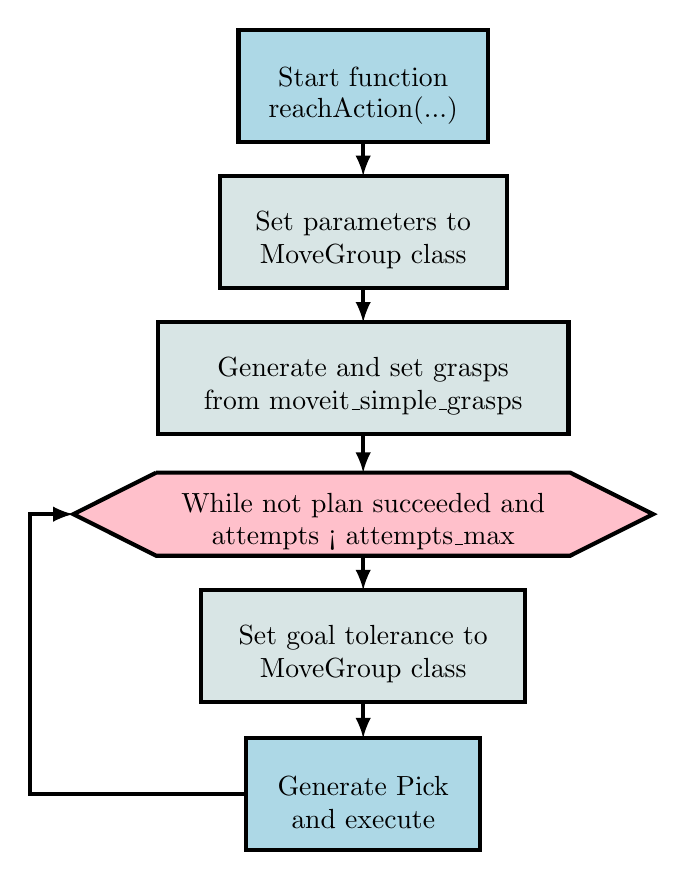
\begin{tikzpicture}
\pgftransformxscale{1.000000}
\pgftransformyscale{-1.000000}
\definecolor{dialinecolor}{rgb}{0.000000, 0.000000, 0.000000}
\pgfsetstrokecolor{dialinecolor}
\definecolor{dialinecolor}{rgb}{1.000000, 1.000000, 1.000000}
\pgfsetfillcolor{dialinecolor}
\definecolor{dialinecolor}{rgb}{0.678431, 0.847059, 0.901961}
\pgfsetfillcolor{dialinecolor}
\fill (12.266500\du,3.050000\du)--(12.266500\du,5.750000\du)--(18.271500\du,5.750000\du)--(18.271500\du,3.050000\du)--cycle;
\pgfsetlinewidth{0.100000\du}
\pgfsetdash{}{0pt}
\pgfsetdash{}{0pt}
\pgfsetmiterjoin
\definecolor{dialinecolor}{rgb}{0.000000, 0.000000, 0.000000}
\pgfsetstrokecolor{dialinecolor}
\draw (12.266500\du,3.050000\du)--(12.266500\du,5.750000\du)--(18.271500\du,5.750000\du)--(18.271500\du,3.050000\du)--cycle;
% setfont left to latex
\definecolor{dialinecolor}{rgb}{0.000000, 0.000000, 0.000000}
\pgfsetstrokecolor{dialinecolor}
\node at (15.269000\du,4.195000\du){Start function};
% setfont left to latex
\definecolor{dialinecolor}{rgb}{0.000000, 0.000000, 0.000000}
\pgfsetstrokecolor{dialinecolor}
\node at (15.269000\du,4.995000\du){reachAction(...)};
\definecolor{dialinecolor}{rgb}{0.847059, 0.898039, 0.898039}
\pgfsetfillcolor{dialinecolor}
\fill (11.812750\du,6.570710\du)--(11.812750\du,9.270710\du)--(18.725250\du,9.270710\du)--(18.725250\du,6.570710\du)--cycle;
\pgfsetlinewidth{0.100000\du}
\pgfsetdash{}{0pt}
\pgfsetdash{}{0pt}
\pgfsetmiterjoin
\definecolor{dialinecolor}{rgb}{0.000000, 0.000000, 0.000000}
\pgfsetstrokecolor{dialinecolor}
\draw (11.812750\du,6.570710\du)--(11.812750\du,9.270710\du)--(18.725250\du,9.270710\du)--(18.725250\du,6.570710\du)--cycle;
% setfont left to latex
\definecolor{dialinecolor}{rgb}{0.000000, 0.000000, 0.000000}
\pgfsetstrokecolor{dialinecolor}
\node at (15.269000\du,7.715710\du){Set parameters to};
% setfont left to latex
\definecolor{dialinecolor}{rgb}{0.000000, 0.000000, 0.000000}
\pgfsetstrokecolor{dialinecolor}
\node at (15.269000\du,8.515710\du){MoveGroup class};
\pgfsetlinewidth{0.100000\du}
\pgfsetdash{}{0pt}
\pgfsetdash{}{0pt}
\pgfsetbuttcap
\pgfsetmiterjoin
\pgfsetlinewidth{0.100000\du}
\pgfsetbuttcap
\pgfsetmiterjoin
\pgfsetdash{}{0pt}
\definecolor{dialinecolor}{rgb}{1.000000, 0.752941, 0.796078}
\pgfsetfillcolor{dialinecolor}
\pgfpathmoveto{\pgfpoint{10.281500\du}{13.719707\du}}
\pgfpathlineto{\pgfpoint{20.256500\du}{13.719707\du}}
\pgfpathlineto{\pgfpoint{22.251500\du}{14.719707\du}}
\pgfpathlineto{\pgfpoint{20.256500\du}{15.719707\du}}
\pgfpathlineto{\pgfpoint{10.281500\du}{15.719707\du}}
\pgfpathlineto{\pgfpoint{8.286500\du}{14.719707\du}}
\pgfpathlineto{\pgfpoint{10.281500\du}{13.719707\du}}
\pgfusepath{fill}
\definecolor{dialinecolor}{rgb}{0.000000, 0.000000, 0.000000}
\pgfsetstrokecolor{dialinecolor}
\pgfpathmoveto{\pgfpoint{10.281500\du}{13.719707\du}}
\pgfpathlineto{\pgfpoint{20.256500\du}{13.719707\du}}
\pgfpathlineto{\pgfpoint{22.251500\du}{14.719707\du}}
\pgfpathlineto{\pgfpoint{20.256500\du}{15.719707\du}}
\pgfpathlineto{\pgfpoint{10.281500\du}{15.719707\du}}
\pgfpathlineto{\pgfpoint{8.286500\du}{14.719707\du}}
\pgfpathlineto{\pgfpoint{10.281500\du}{13.719707\du}}
\pgfusepath{stroke}
% setfont left to latex
\definecolor{dialinecolor}{rgb}{0.000000, 0.000000, 0.000000}
\pgfsetstrokecolor{dialinecolor}
\node at (15.269000\du,14.519707\du){While not plan succeeded and};
% setfont left to latex
\definecolor{dialinecolor}{rgb}{0.000000, 0.000000, 0.000000}
\pgfsetstrokecolor{dialinecolor}
\node at (15.269000\du,15.319707\du){attempts < attempts\_max};
\definecolor{dialinecolor}{rgb}{0.847059, 0.898039, 0.898039}
\pgfsetfillcolor{dialinecolor}
\fill (11.371500\du,16.549007\du)--(11.371500\du,19.249007\du)--(19.166500\du,19.249007\du)--(19.166500\du,16.549007\du)--cycle;
\pgfsetlinewidth{0.100000\du}
\pgfsetdash{}{0pt}
\pgfsetdash{}{0pt}
\pgfsetmiterjoin
\definecolor{dialinecolor}{rgb}{0.000000, 0.000000, 0.000000}
\pgfsetstrokecolor{dialinecolor}
\draw (11.371500\du,16.549007\du)--(11.371500\du,19.249007\du)--(19.166500\du,19.249007\du)--(19.166500\du,16.549007\du)--cycle;
% setfont left to latex
\definecolor{dialinecolor}{rgb}{0.000000, 0.000000, 0.000000}
\pgfsetstrokecolor{dialinecolor}
\node at (15.269000\du,17.694007\du){Set goal tolerance to};
% setfont left to latex
\definecolor{dialinecolor}{rgb}{0.000000, 0.000000, 0.000000}
\pgfsetstrokecolor{dialinecolor}
\node at (15.269000\du,18.494007\du){MoveGroup class};
\definecolor{dialinecolor}{rgb}{0.678431, 0.847059, 0.901961}
\pgfsetfillcolor{dialinecolor}
\fill (12.446056\du,20.115808\du)--(12.446056\du,22.815808\du)--(18.091944\du,22.815808\du)--(18.091944\du,20.115808\du)--cycle;
\pgfsetlinewidth{0.100000\du}
\pgfsetdash{}{0pt}
\pgfsetdash{}{0pt}
\pgfsetmiterjoin
\definecolor{dialinecolor}{rgb}{0.000000, 0.000000, 0.000000}
\pgfsetstrokecolor{dialinecolor}
\draw (12.446056\du,20.115808\du)--(12.446056\du,22.815808\du)--(18.091944\du,22.815808\du)--(18.091944\du,20.115808\du)--cycle;
% setfont left to latex
\definecolor{dialinecolor}{rgb}{0.000000, 0.000000, 0.000000}
\pgfsetstrokecolor{dialinecolor}
\node at (15.269000\du,21.260808\du){Generate Pick};
% setfont left to latex
\definecolor{dialinecolor}{rgb}{0.000000, 0.000000, 0.000000}
\pgfsetstrokecolor{dialinecolor}
\node at (15.269000\du,22.060808\du){and execute};
\pgfsetlinewidth{0.100000\du}
\pgfsetdash{}{0pt}
\pgfsetdash{}{0pt}
\pgfsetbuttcap
{
\definecolor{dialinecolor}{rgb}{0.000000, 0.000000, 0.000000}
\pgfsetfillcolor{dialinecolor}
% was here!!!
\pgfsetarrowsend{latex}
\definecolor{dialinecolor}{rgb}{0.000000, 0.000000, 0.000000}
\pgfsetstrokecolor{dialinecolor}
\draw (15.269000\du,5.750000\du)--(15.269000\du,6.570710\du);
}
\pgfsetlinewidth{0.100000\du}
\pgfsetdash{}{0pt}
\pgfsetdash{}{0pt}
\pgfsetbuttcap
{
\definecolor{dialinecolor}{rgb}{0.000000, 0.000000, 0.000000}
\pgfsetfillcolor{dialinecolor}
% was here!!!
\pgfsetarrowsend{latex}
\definecolor{dialinecolor}{rgb}{0.000000, 0.000000, 0.000000}
\pgfsetstrokecolor{dialinecolor}
\draw (15.269000\du,15.719707\du)--(15.269000\du,16.549007\du);
}
\pgfsetlinewidth{0.100000\du}
\pgfsetdash{}{0pt}
\pgfsetdash{}{0pt}
\pgfsetbuttcap
{
\definecolor{dialinecolor}{rgb}{0.000000, 0.000000, 0.000000}
\pgfsetfillcolor{dialinecolor}
% was here!!!
\pgfsetarrowsend{latex}
\definecolor{dialinecolor}{rgb}{0.000000, 0.000000, 0.000000}
\pgfsetstrokecolor{dialinecolor}
\draw (15.269000\du,19.298579\du)--(15.269000\du,20.115808\du);
}
\pgfsetlinewidth{0.100000\du}
\pgfsetdash{}{0pt}
\pgfsetdash{}{0pt}
\pgfsetmiterjoin
\pgfsetbuttcap
{
\definecolor{dialinecolor}{rgb}{0.000000, 0.000000, 0.000000}
\pgfsetfillcolor{dialinecolor}
% was here!!!
\pgfsetarrowsend{latex}
{\pgfsetcornersarced{\pgfpoint{0.000000\du}{0.000000\du}}\definecolor{dialinecolor}{rgb}{0.000000, 0.000000, 0.000000}
\pgfsetstrokecolor{dialinecolor}
\draw (12.446056\du,21.465808\du)--(7.236500\du,21.465808\du)--(7.236500\du,14.719707\du)--(8.286500\du,14.719707\du);
}}
\pgfsetlinewidth{0.100000\du}
\pgfsetdash{}{0pt}
\pgfsetdash{}{0pt}
\pgfsetbuttcap
{
\definecolor{dialinecolor}{rgb}{0.000000, 0.000000, 0.000000}
\pgfsetfillcolor{dialinecolor}
% was here!!!
\pgfsetarrowsend{latex}
\definecolor{dialinecolor}{rgb}{0.000000, 0.000000, 0.000000}
\pgfsetstrokecolor{dialinecolor}
\draw (15.269000\du,12.796933\du)--(15.269000\du,13.719707\du);
}
\pgfsetlinewidth{0.100000\du}
\pgfsetdash{}{0pt}
\pgfsetdash{}{0pt}
\pgfsetbuttcap
{
\definecolor{dialinecolor}{rgb}{0.000000, 0.000000, 0.000000}
\pgfsetfillcolor{dialinecolor}
% was here!!!
\pgfsetarrowsend{latex}
\definecolor{dialinecolor}{rgb}{0.000000, 0.000000, 0.000000}
\pgfsetstrokecolor{dialinecolor}
\draw (15.269000\du,9.270710\du)--(15.269000\du,10.096933\du);
}
\definecolor{dialinecolor}{rgb}{0.847059, 0.898039, 0.898039}
\pgfsetfillcolor{dialinecolor}
\fill (10.321500\du,10.096933\du)--(10.321500\du,12.796933\du)--(20.216500\du,12.796933\du)--(20.216500\du,10.096933\du)--cycle;
\pgfsetlinewidth{0.100000\du}
\pgfsetdash{}{0pt}
\pgfsetdash{}{0pt}
\pgfsetmiterjoin
\definecolor{dialinecolor}{rgb}{0.000000, 0.000000, 0.000000}
\pgfsetstrokecolor{dialinecolor}
\draw (10.321500\du,10.096933\du)--(10.321500\du,12.796933\du)--(20.216500\du,12.796933\du)--(20.216500\du,10.096933\du)--cycle;
% setfont left to latex
\definecolor{dialinecolor}{rgb}{0.000000, 0.000000, 0.000000}
\pgfsetstrokecolor{dialinecolor}
\node at (15.269000\du,11.241933\du){Generate and set grasps};
% setfont left to latex
\definecolor{dialinecolor}{rgb}{0.000000, 0.000000, 0.000000}
\pgfsetstrokecolor{dialinecolor}
\node at (15.269000\du,12.041933\du){from moveit\_simple\_grasps};
\end{tikzpicture}
